\section*{HSR's Software and External Devices}
% In this section briefly describe the software and hardware of the robot

\setlength\intextsep{0pt}
\begin{wrapfigure}[5]{r}{0.3\textwidth}
	\centering
	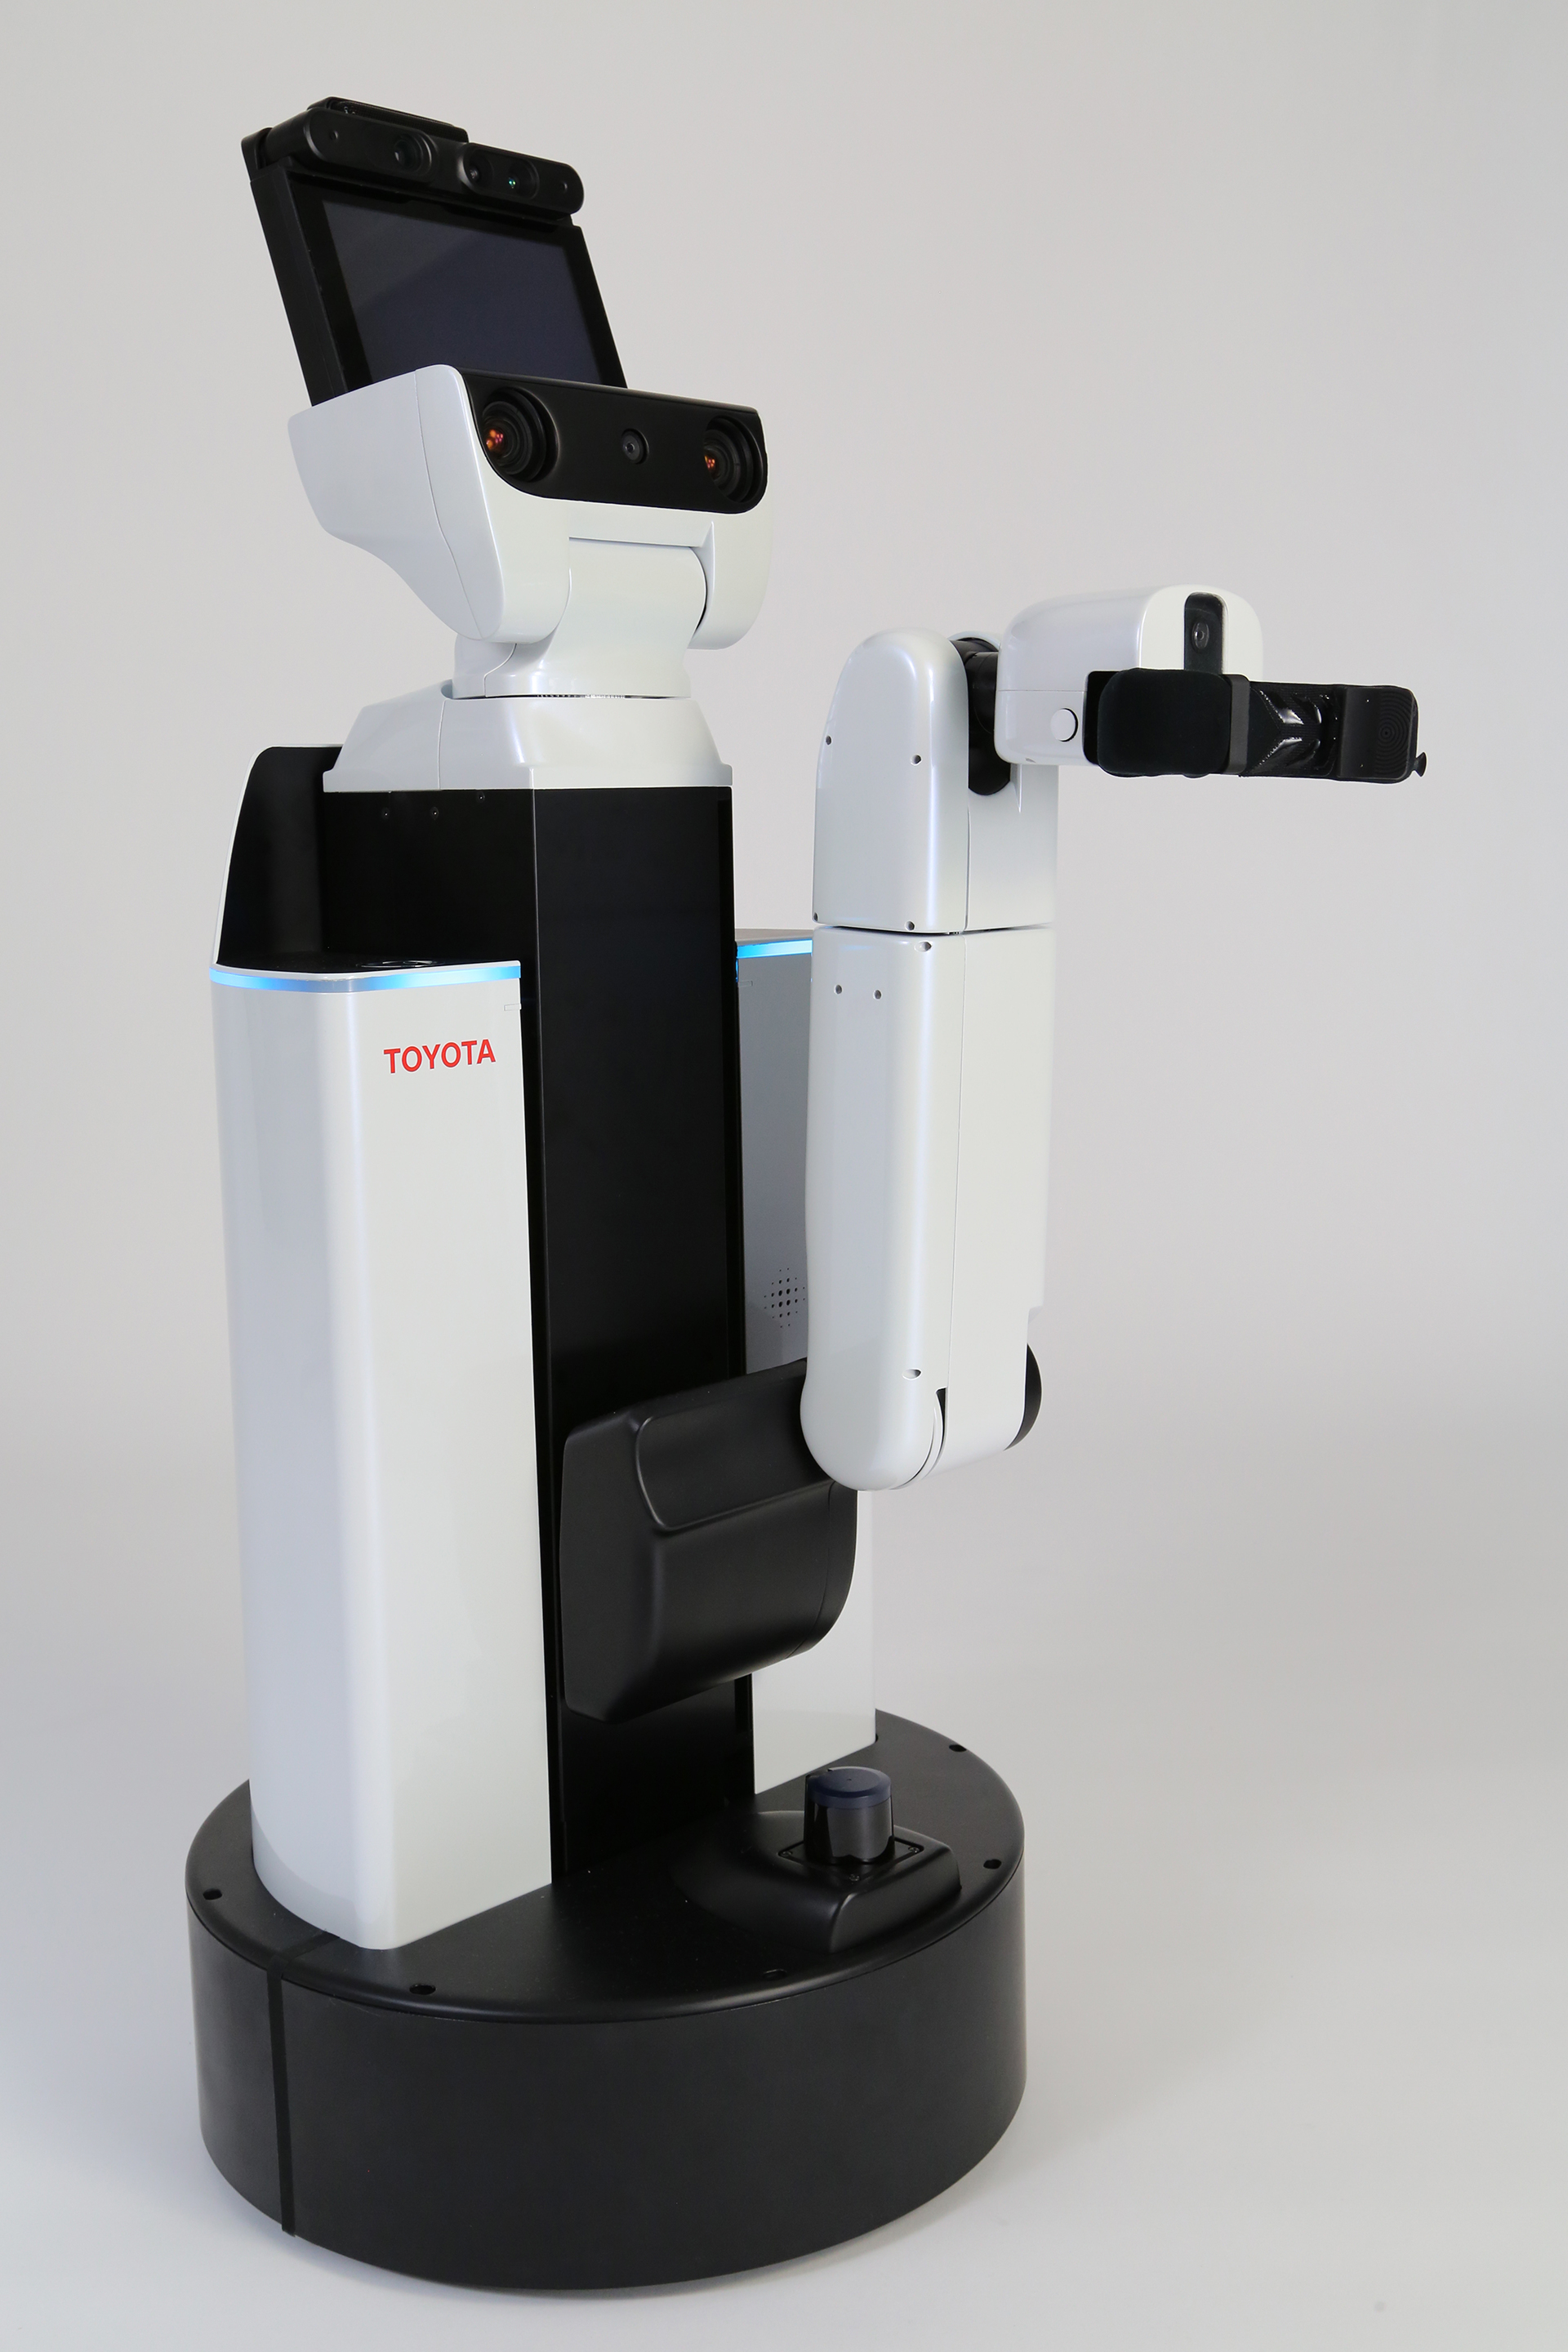
\includegraphics[width=0.3\textwidth]{Toyota_HSR}
	\caption{The Toyota HSR Robot, HERO}
	\label{fig:hsr}
\end{wrapfigure}

We use a standard \textit{Toyota} HSR robot unit. To differentiate our unit, we named it HERO. We wanted to link the name to our AMIGO and SERGIO domestic service robots.

\section*{HERO's Software Description}
% Please describe in this section the software you are using to control your robot. Consider the following example:

An overview of the software used by the Tech United Eindhoven @Home robots can be found in Table~\ref{tab:softwarespec}.
All our software is developed open-source at GitHub\footnote{\url{https://github.com/tue-robotics}}.
\\\newline
Currently, we have some \textit{image\_recognition} packages released into the current ROS Kinetic distribution and can be installed with use of \textit{apt}.

\begin{table}[H]
    \begin{center}
    \caption{Software overview of the robots.}
    \label{tab:softwarespec}
    %\vspace{-0.1cm}
    \renewcommand{\arraystretch}{1.0}
    \setlength{\tabcolsep}{5pt}
        \begin{tabular}{p{0.3\textwidth} p{0.7\textwidth}}
            \toprule
            Operating system & Ubuntu 16.04 LTS Server\\

            Middleware & ROS Kinetic~\cite{Quigley2009}\\

            Low-level control software & Orocos Real-Time Toolkit~\cite{Bruyninckx2001}\newline
            \url{https://github.com/tue-robotics/rtt_control_components}
            \\

            Simulation & Custom kinematics + sensor simulator \newline
            \url{https://github.com/tue-robotics/fast_simulator}
            \\

            World model & \acrfull{ed}, custom \newline
            \url{https://github.com/tue-robotics/ed}\\

            Localization & Monte Carlo~\cite{Fox2003} using \gls{ed}, custom \newline \url{https://github.com/tue-robotics/ed\_localization}\\

            SLAM & Gmapping package \newline \url{http://wiki.ros.org/gmapping}\\

            Navigation & CB Base navigation
            \newline
            \url{https://github.com/tue-robotics/cb_base_navigation}
            \newline
            Global: custom A* planner\newline Local: modified ROS DWA~\cite{Fox1997}\\

            Arm navigation & Custom implementation using MoveIt and Orocos KDL\newline
            \url{https://github.com/tue-robotics/tue_manipulation}
            \\

            Object recognition & Tensorflow ROS \newline
			\url{https://github.com/tue-robotics/image\_recognition/tree/master/tensorflow\_ros}\\

            People detection & Custom implementation using contour matching \newline
            \url{https://github.com/tue-robotics/ed_perception}
            \\
            Face detection \& recognition & Openface ROS \newline \url{https://github.com/tue-robotics/image\_recognition/tree/master/openface\_ros} \\

            Speech recognition & Julius Speech Recognition \newline
            \url{https://github.com/julius-speech/julius}\\
            Speech synthesis & Toyota\texttrademark \hspace{0em} Text-to-Speech\\
            Task executors & SMACH \newline
            \url{https://github.com/tue-robotics/tue_robocup}\\
            \bottomrule
        \end{tabular}
    \end{center}
\end{table}

This our current software implementation on our robots AMIGO and SERGIO, which participate in the open league. Because of the pending delivery of the Toyota HSR and related documentation, we are not able to provide the specific software implementation. As described in our selection qualification paper, our goal is to use the same software as possible on all our robots, including the Toyota HSR.

\section*{External Devices}
% Please describe in this section the external devices used by your robot. Consider the following example:

\textit{HERO relies on the following external hardware:}

\begin{itemize}
	\item Mother-ship
	\item Data Cluster
	\item $3 \times$ Ultra-Power laptops.
\end{itemize}

\section*{Cloud Services}
% Please describe in this section the Cloud Services and online software used by your robot. Consider the following example:

\textit{HERO connects the following cloud services:}
\begin{itemize}
	\item Localization and mapping: Geolocalization system.
	\item Navigation: Navigator
	\item Speech recognition: All-purpose recognizer.
\end{itemize} 